\documentclass[tikz]{standalone}

\usetikzlibrary{calc}

\tikzset{signal/.style={%
  ->,
  very thick,
  >=latex,
  rounded corners,
  }
}

\tikzset{block/.style={%
  inner sep=2mm,
  anchor=center,
  rounded corners,
  very thick,
  draw,
  }
}

\tikzset{block diagram/.style={every path/.style={signal},every node/.style={block,draw=none}}}
\tikzstyle{input} = [coordinate]
\tikzstyle{output} = [coordinate]
\begin{document}

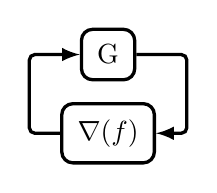
\begin{tikzpicture}[block diagram]
  
  \node (system) [block] {G};
  
  \node (grad) [block, below of=system] {\( \nabla (f) \)};

  \coordinate [right of=system] (tmp1);
  \coordinate [right of=grad] (tmp2); 
  \coordinate [left of=grad] (tmp3);
  \coordinate [left of=system] (tmp4);
  

  \draw [->, rounded corners=2pt] (system.east) -- (tmp1) -- (tmp2) -- (grad); 
  \draw [->, rounded corners=2pt] (grad.west) -- (tmp3) -- (tmp4) -- (system); 
\end{tikzpicture}

\end{document}
